\documentclass[10pt,a4paper]{report}
\usepackage[utf8]{inputenc}
\usepackage[T1]{fontenc}
\usepackage{amsmath}
\usepackage{amsfonts}
\usepackage{amssymb}
\usepackage{makeidx}
\usepackage{graphicx}
\usepackage{xcolor}
\usepackage{tikz,pgf}
\begin{document}
	\begin{center}
		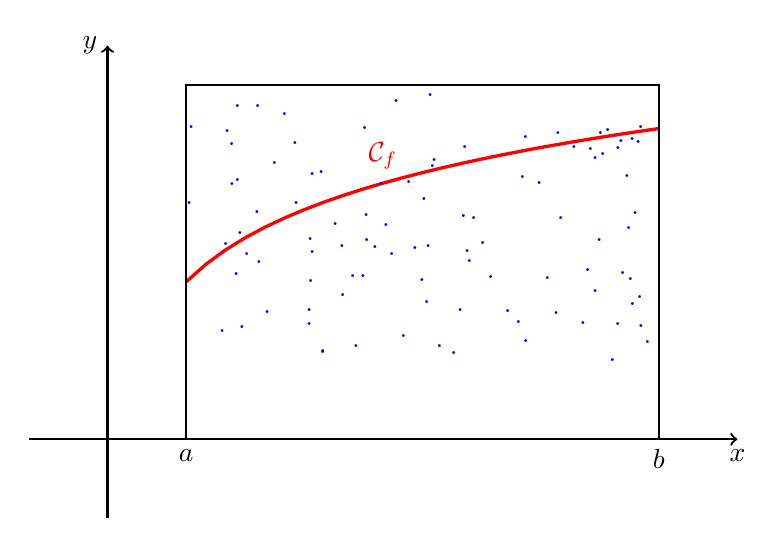
\begin{tikzpicture}[scale=1]
			\draw[->=latex,thick](-1,0)--(8,0)node[below]{$ x $};
			\draw[->=latex,thick](0,-1)--(0,5)node[left]{$ y $};
			\draw[thick](3.5,3.6)node[red]{$ \mathcal{C}_{f} $};
			\draw[red,very thick][domain=1:7]plot(\x,{2+ln(\x)});
			\draw[thick](1,0)--(1,4.5)--(7,4.5)--(7,0);
			\draw[thick](1,0)node[below]{$ a $};
			\draw[thick](7,0)node[below]{$ b $};
			\foreach \i in {1,...,100}
			\draw[ very thick,blue](3*rand+4,1.75*rand+2.75)node{.};
		\end{tikzpicture}
	\end{center}
\end{document}